\documentclass{article}
\usepackage[utf8]{inputenc}
\usepackage[greek,english]{babel}
\usepackage{alphabeta}
\usepackage{fancyhdr}
\usepackage{listings}
\usepackage{mathtools}
\usepackage{xcolor}
\usepackage{biblatex}
\usepackage[left=1cm,right=1cm]{geometry}

\lstset {
        basicstyle=\ttfamily,
        columns=fullflexible,
        breaklines=true,
        keepspaces=true,
	showstringspaces=false
}

\title{Εργαστήριο Παράλληλων Συστημάτων - Εργασία 2}
\author{Χρήστος Μαργιώλης}
\date{Ιανουάριος 2023}

\begin{document}

\begin{titlepage}
        \maketitle
\end{titlepage}

\renewcommand{\contentsname}{Περιεχόμενα}
\tableofcontents
\pagebreak

\section{Προγράμματα}

Οι κώδικες έχουν σχόλια μόνο στα σημεία που θεώρησα ότι μπορεί να προκύψει
κάποιο «μπέρδεμα».

\subsection{'Ασκηση 2Α}

\subsubsection{Κώδικας}
\lstinputlisting[language=C]{ex2a.c}
\pagebreak
\subsubsection{Ενδεικτικά τρεξίματα}

\begin{lstlisting}
usage: ./a.out nthreads n
\end{lstlisting}

Για \lstinline{nthreads = 2} και \lstinline{n = 10}: \\

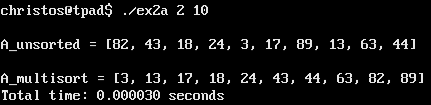
\includegraphics[width=\textwidth]{res/ex2a_1.png} \\

Για \lstinline{nthreads = 8} και \lstinline{n = 100}: \\

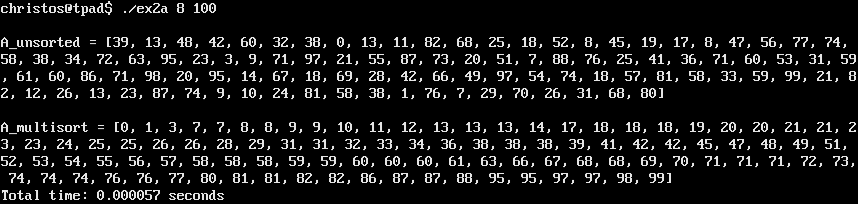
\includegraphics[width=\textwidth]{res/ex2a_2.png} \\

Για \lstinline{nthreads = 16} και \lstinline{n = 1000000}. Λόγω του αριθμού των
στοιχείων, το στιγμιότυπο δείχνει μόνο τον χρόνο υπολογισμού: \\


\includegraphics[width=\textwidth]{res/ex2a_3.png} \\
\pagebreak

\subsection{'Ασκηση 2Β-Α}

\subsubsection{Κώδικας}
\lstinputlisting[language=C]{ex2b_a.cu}
\pagebreak
\subsubsection{Ενδεικτικά τρεξίματα}

Για \lstinline{NxN = 8x8} και \lstinline{blocksize = 256} \\

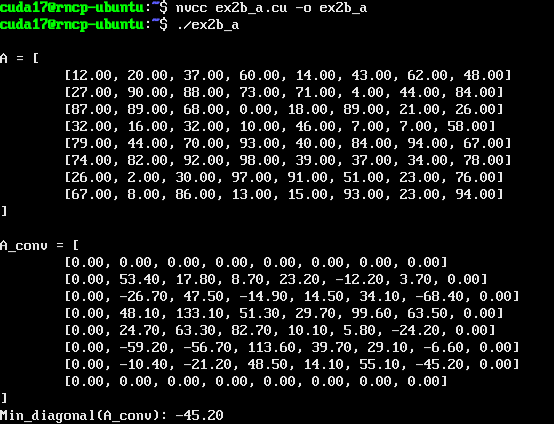
\includegraphics[width=\textwidth]{res/ex2b_a_1.png} \\

Για \lstinline{NxN = 32x32} και \lstinline{blocksize = 1024} \\

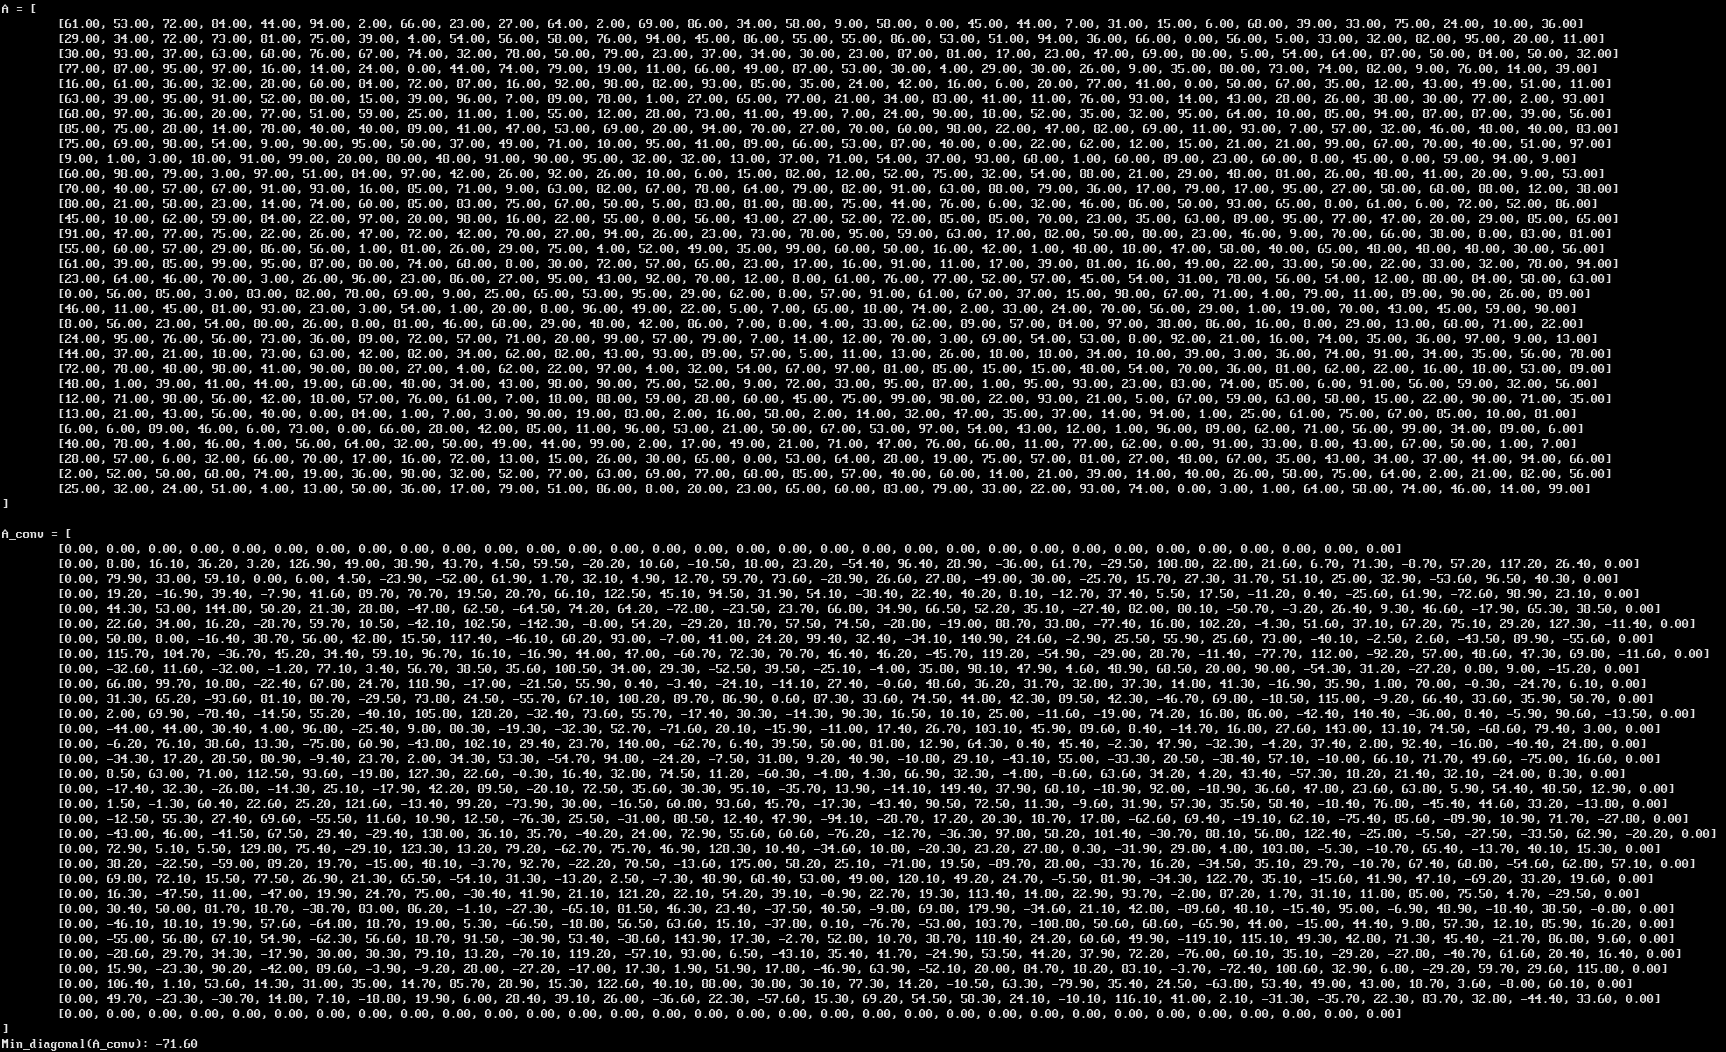
\includegraphics[width=\textwidth]{res/ex2b_a_2.png} \\

Για \lstinline{NxN = 4x4} και \lstinline{blocksize = 256} \\

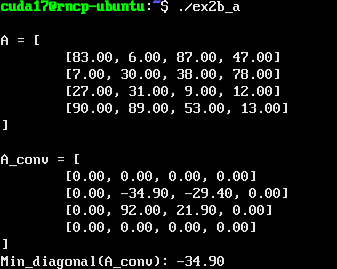
\includegraphics[width=\textwidth]{res/ex2b_a_3.png} \\
\pagebreak

\subsection{'Ασκηση 2Β-Β}

\subsubsection{Κώδικας}
\lstinputlisting[language=C]{ex2b_b.cu}
\pagebreak
\subsubsection{Ενδεικτικά τρεξίματα}

Για \lstinline{NxM = 4x2} και \lstinline{blocksize = 256} \\

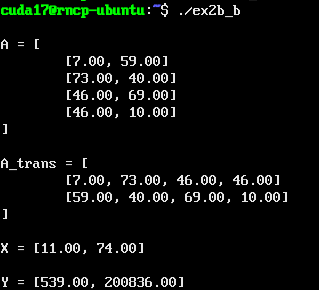
\includegraphics[width=\textwidth]{res/ex2b_b_1.png} \\

Για \lstinline{NxM = 4x8} και \lstinline{blocksize = 256} \\

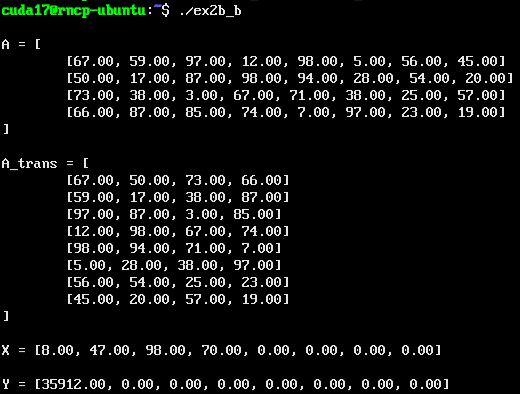
\includegraphics[width=\textwidth]{res/ex2b_b_2.png} \\

Για \lstinline{NxM = 8x8} και \lstinline{blocksize = 1024} \\

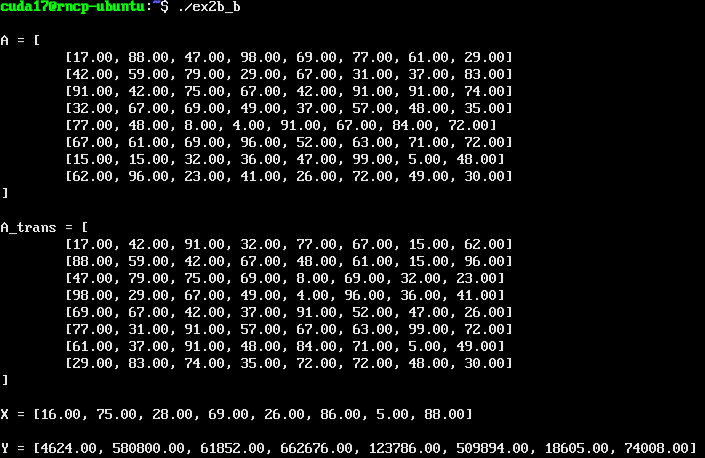
\includegraphics[width=\textwidth]{res/ex2b_b_3.png} \\

\section{Προβλήματα}

Δεν υλοποίησα την άσκηση 2B-Γ (συνδιακύμανση).

\end{document}
